
%----------------------------------------------------------------------------------------
%	SECTION 2
%----------------------------------------------------------------------------------------

\section{Arup, August 2016}

%\subsection{Mechanical Engineering Summer Placement at Arup in Leeds}

In the summer after second year, I was excited to have earned a mechanical engineering placement with the world-renowned company, Arup, in Leeds' Buildings team.
I was responsible for sizing ducts and pipes and for producing the RIBA Stage 3 layouts and schematics of a new-build’s ventilation, heating and domestic water systems (see Figure \ref{fig:arup_schematics}).
This placement gave me my first hands-on experience in designing and sizing such systems.
I appreciated the level of responsibility (and its associated challenge) that I was given since Day 1.
I was also introduced to some of the work the electrical engineers did.

The work experience prepared me for future courses such as \textit{Electrical and Lighting Services for Buildings} and the 4\textsuperscript{th} year \textit{Design Project}.
I was encouraged to hear about Arup's sustainable mindset to designing and felt like I could become competent and may enjoy a job as a consulting engineer in the future.


\begin{figure}[htbp]
	\centering
	\begin{subfigure}[b]{0.48\textwidth}
		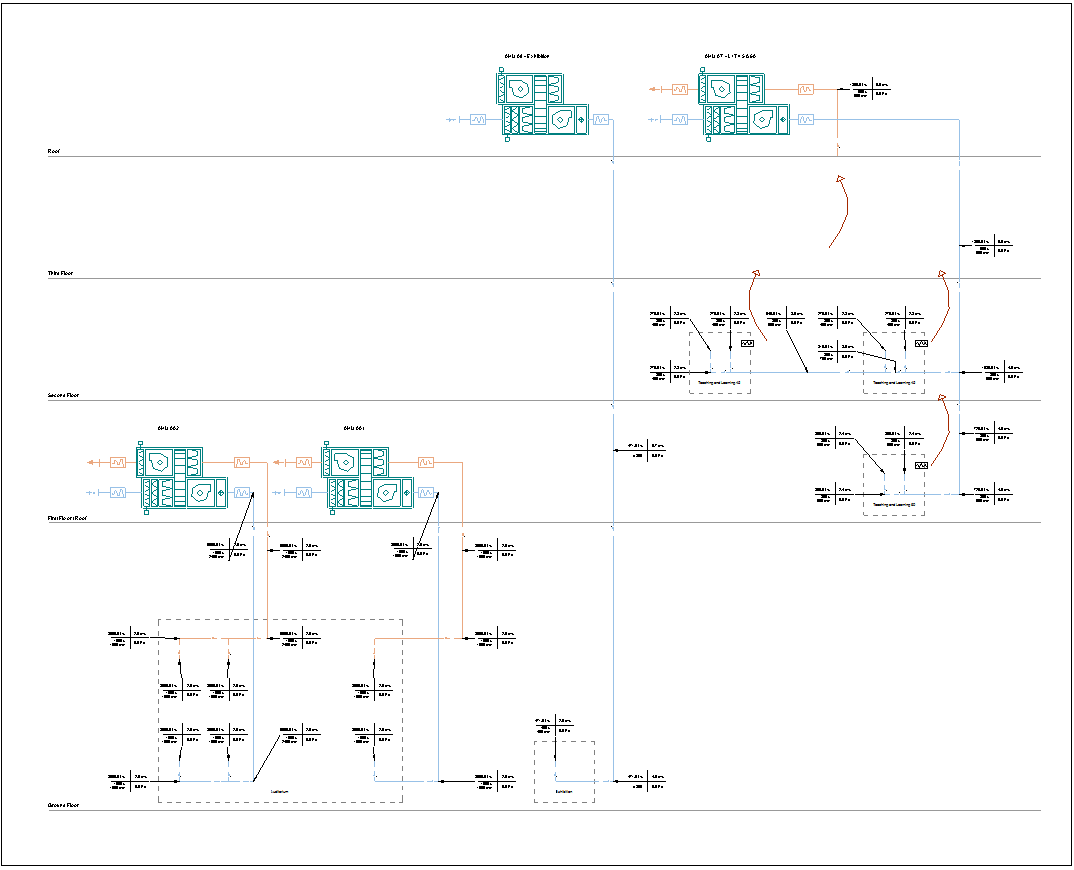
\includegraphics[width=\textwidth]{figures/VentilationSchem3.PNG}
		\caption[Arup ventilation schematic.]{Ventilation schematic.}\label{fig:ventilation}
	\end{subfigure}
	
	\begin{subfigure}[b]{.48\textwidth}
		\centering
		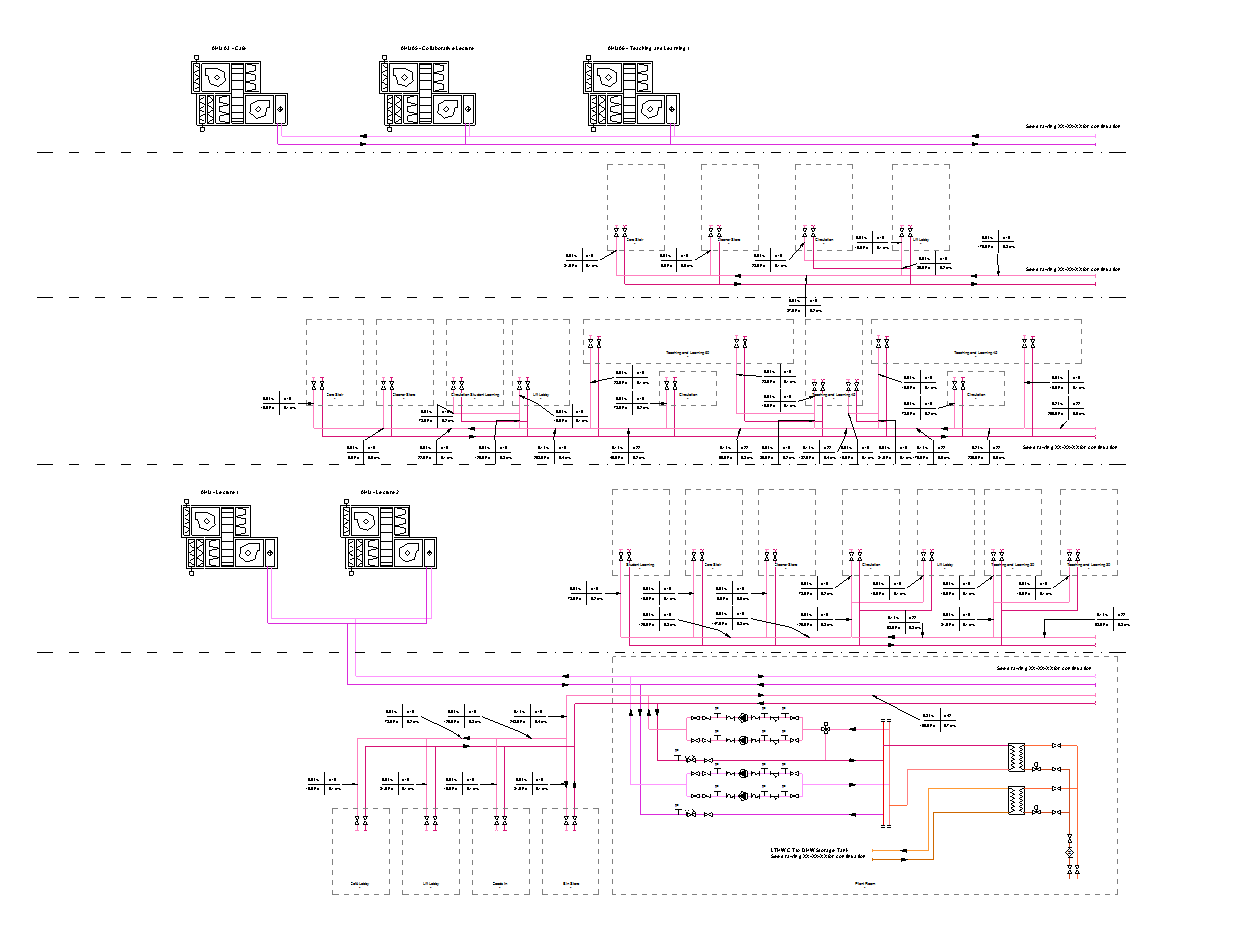
\includegraphics[width=\textwidth]{figures/HeatingSchem.PNG}
		\caption[Arup heating schematic.]{Heating schematic.}\label{fig:heating}
	\end{subfigure}
	\begin{subfigure}[b]{.48\textwidth}
		\centering
		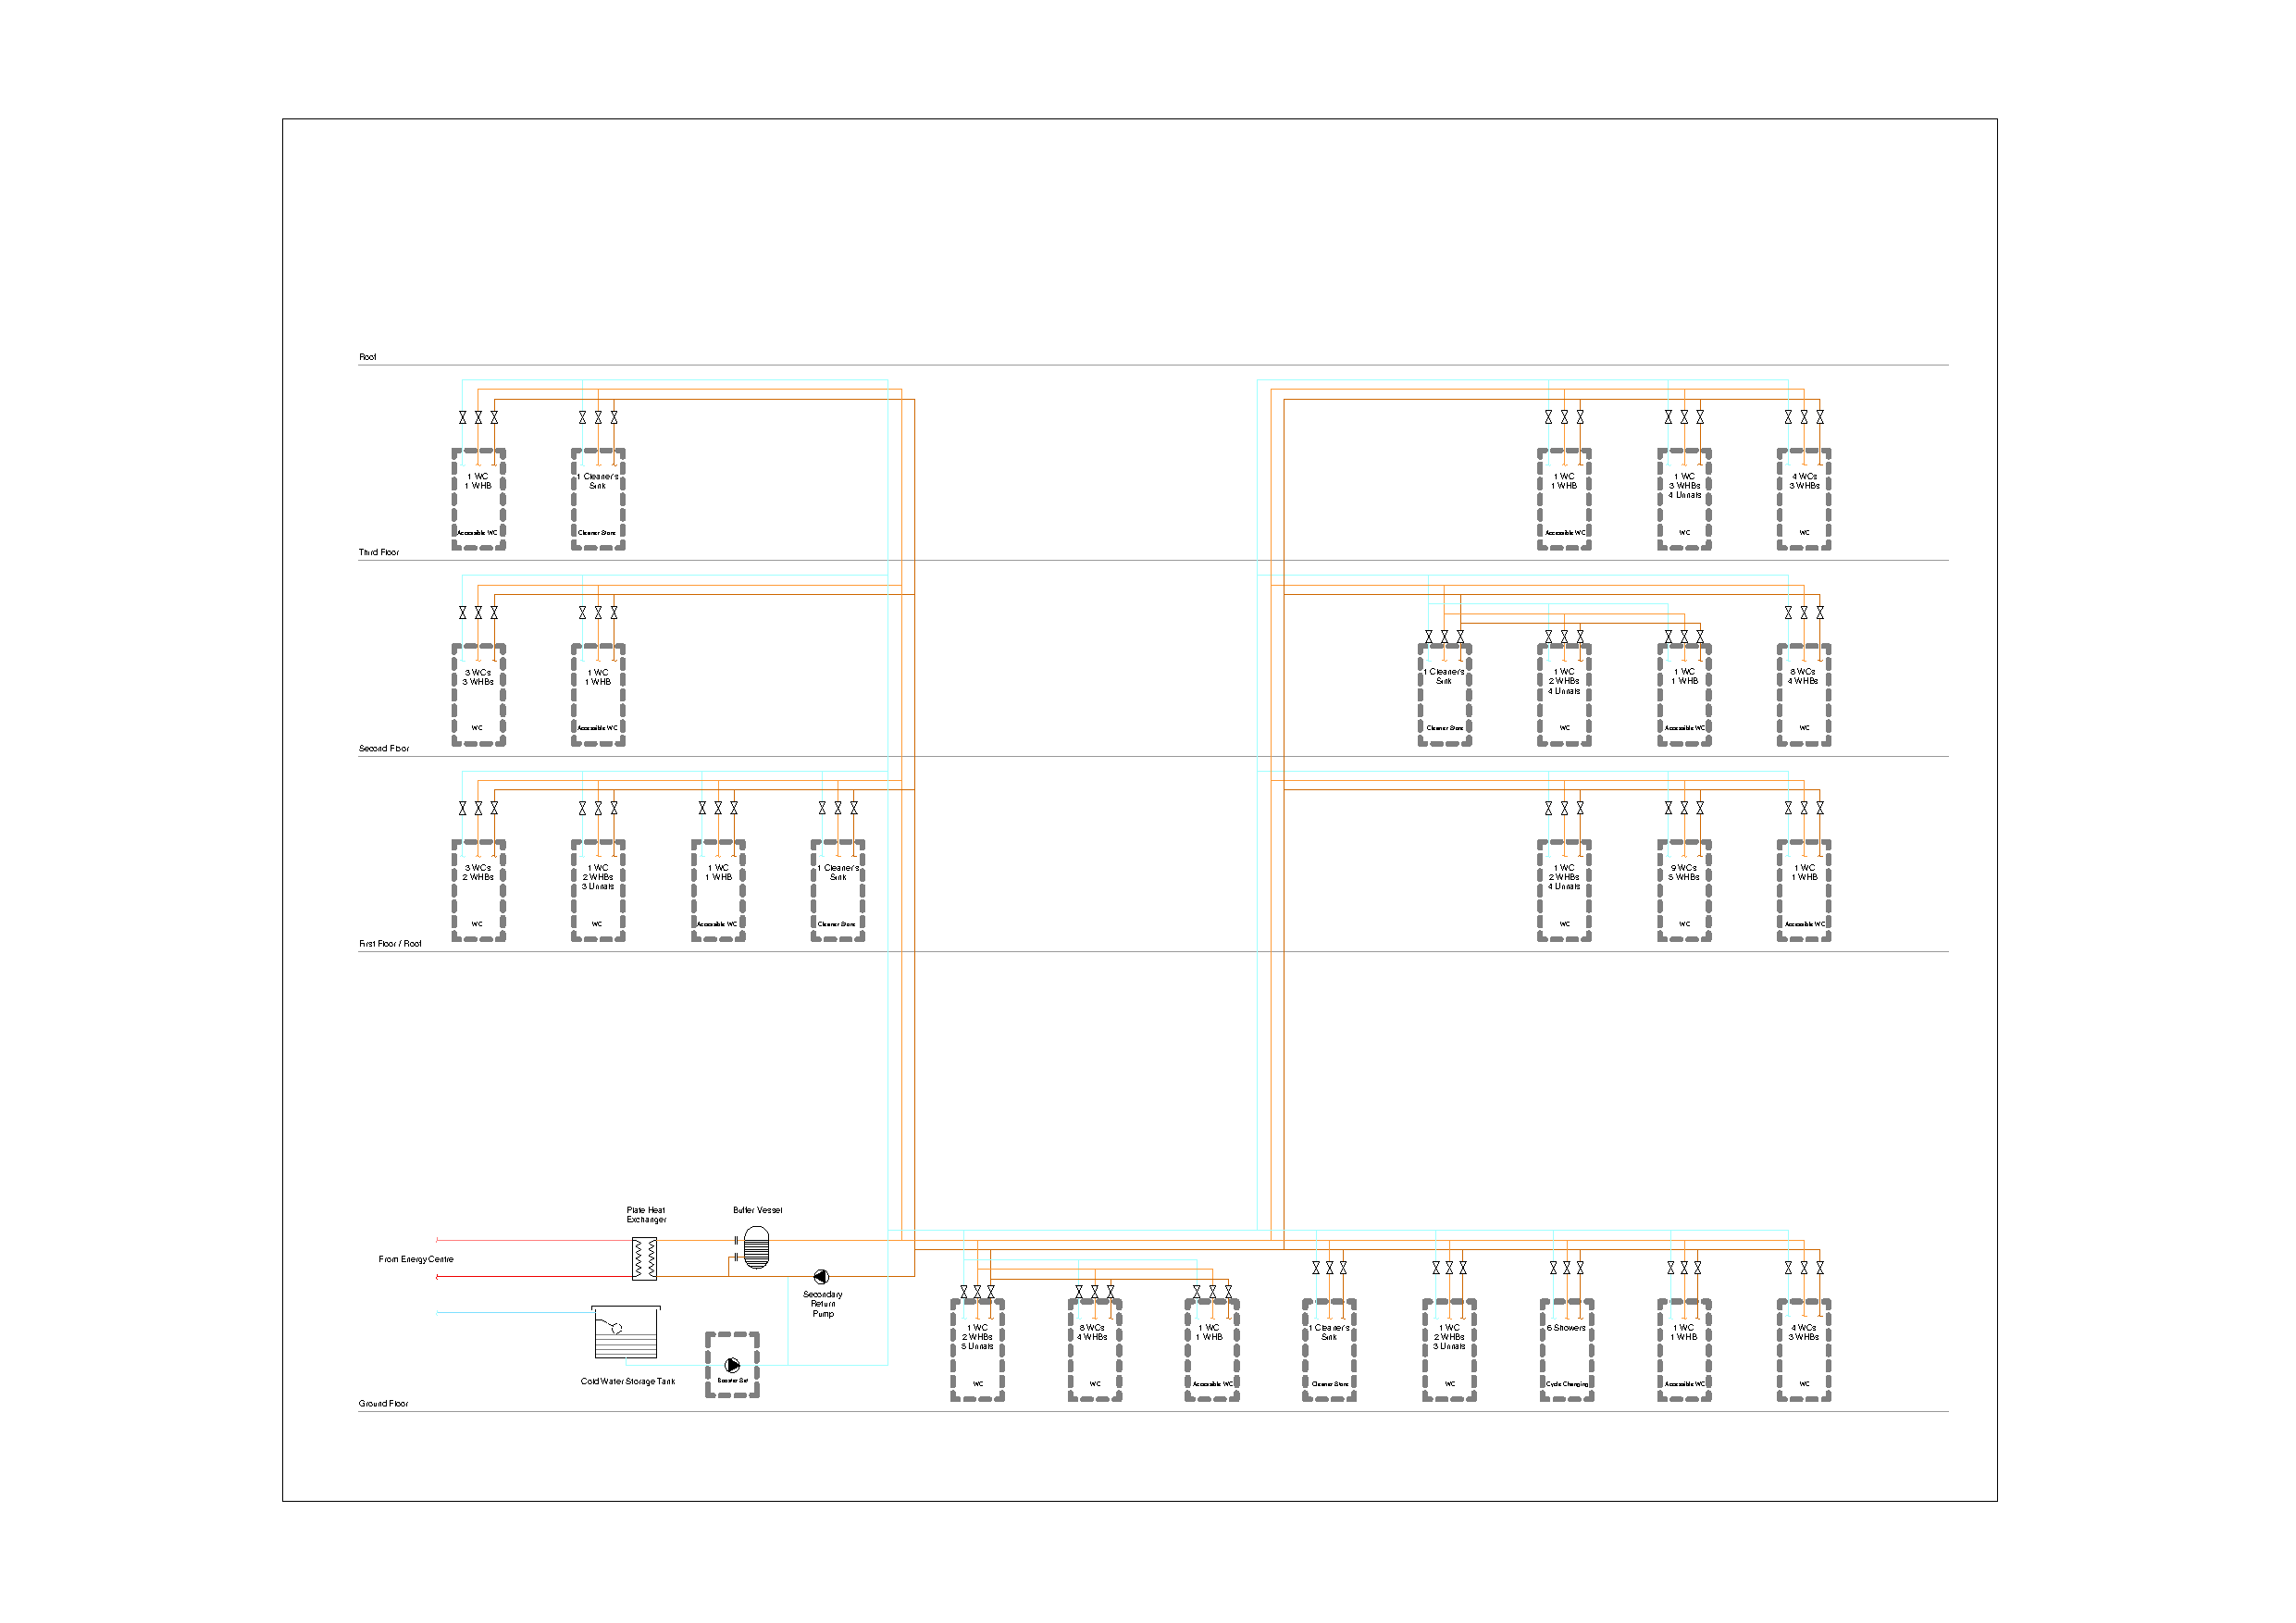
\includegraphics[width=\textwidth]{figures/DomesticsSchem.pdf}
		\caption[Arup domestic schematic.]{Domestic water services schematic.}\label{fig:domestic}
	\end{subfigure}
	\rule{\textwidth}{0.5pt} % use line???
	\caption{Schematics produced at Arup.}
	\label{fig:arup_schematics}
\end{figure}